% 
%
\documentclass[11pt]{article}
\usepackage[pdftex]{graphicx}
\usepackage[utf8]{inputenc}
\usepackage{amssymb}
\usepackage{latexsym}
%\usepackage{relsize}
\usepackage{textcomp}
%processed for 10 pt 
%\documentstyle[epsf,psfig]{article}
%\documentstyle[epsf]{article}
\oddsidemargin 0pt
\topmargin -0.0cm
\textwidth 6.2in
\textheight 8.5in
\baselineskip 18pt
%\renewcommand{\baselinestretch} {1.5}

\newcommand{\fract}[2]{\frac{\textstyle #1}{\textstyle #2}}
\newcommand{\trans}[3]{#1 \stackrel{#2}{\longrightarrow} #3}
\newcommand{\notrans}[3]{#1 \stackrel{#2}{\not\! \longrightarrow} #3}
\bibliographystyle{plain}
\addtocontents{toc}{\setcounter{tocdepth}{2}}
\begin{document}
\title{Handling packet services in Qt-DAB}
\author{
Jan van Katwijk, 
Lazy Chair Computing \\
The Netherlands}

%\date{}
\maketitle
%\baselineskip 22pt
\ \\
DAB transmissions may (and  usually do) carry packet services next to the audio services in an ensemble.
Packet services are in general handled differently from audio services: their
names remain usually invisible to the user, and if a data service runs, it will be in a thread running in the background.

\paragraph{EPG services}
The EPS/SPI service is an obvious example of such a service.
Since the EPG/SPI service - if available - contains Program Guide data
and in many cases {\em icons} of the services in the ensemble,
Qt-DAB automatically detects such a service and starts it (without 
user intervention) as a service running in the background.
An EPG/SPI type service runs in a separate thread and
its output is - invisible to the user - stored, and a directory {\em epg}
in the directory with the Qt-DAB related information.

\paragraph{Displaying the names of data services}
In the default settings for Qt-DAB the names of the data services
(including the EPG/SPI service if available) are {\em not} visible in
the services list.
The {\em configuration and control} window contains
a checkbox selector, labeled {\em show only audio services}, that is set
by default.

\begin{center}
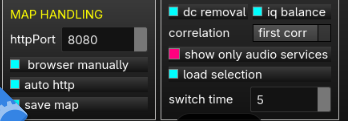
\includegraphics[width=80mm]{checkbox.png}
\end{center}

Unsetting the checkbox and restarting shows all primary services of the
selected ensemble, both audio and packet services. No services of other
ensembles are shown to avoid confusion: names of packet services are qiote
often te same in different ensembles.

\begin{center}
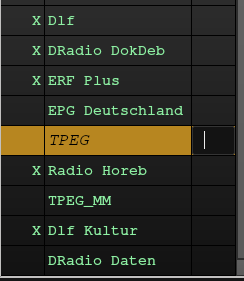
\includegraphics[width=40mm]{servicelist.png}
\end{center}

The {\em content view}, set and unset by clicking with the left mouse button on the ensemblename that is shown above the services list, does show all services, and therefore also the packet services (see below). 

\begin{center}
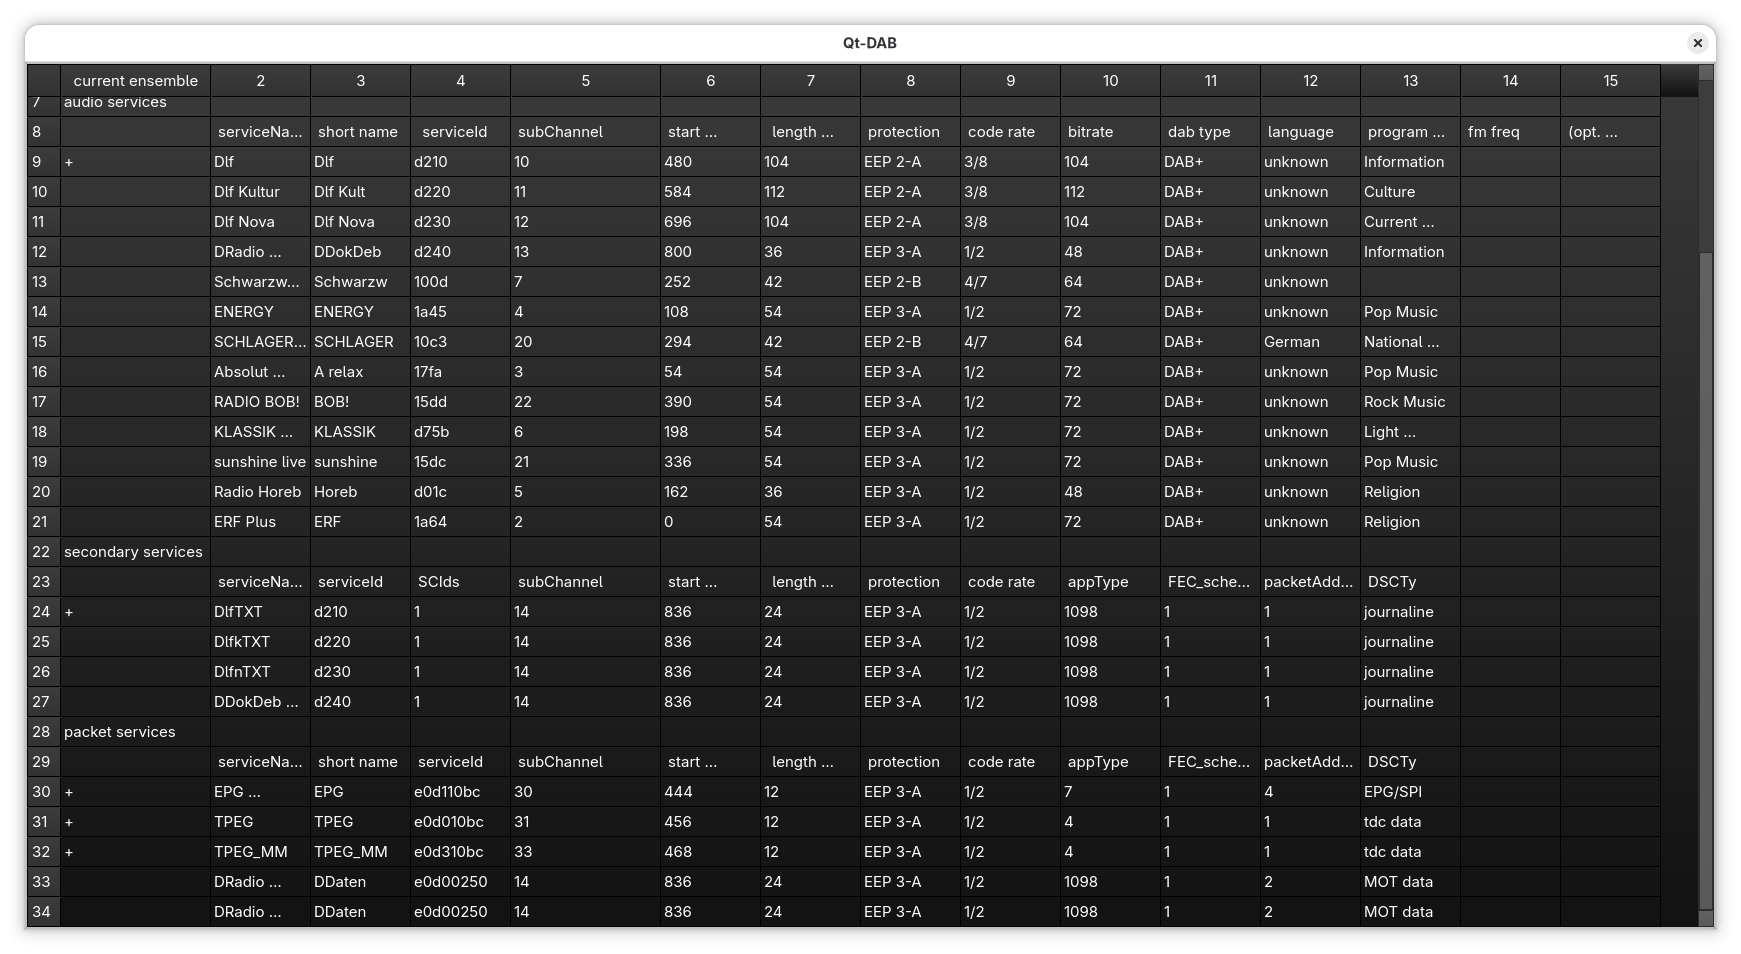
\includegraphics[width=130mm]{content-table.png}
\end{center}

In this particular case, there are three different types of service shown:
\begin{enumerate}
\item the audio services;
\item the {\em secondary} services, i.e. subservices that are automatically activated to run in the background, in this example subservices that display 
{\em journaline} data;
\item the packet services.
\end{enumerate}

The picture shows the EPG service as one of the data services in the ensemble.
The services where a small marker is set in the first column are the ones
that are running in this example.

\paragraph{Running a data service}
Starting a data service is no different from starting any other service,
just click on the name in the servicelist.
Note that clicking on the name of an EPG type service does not have effect, the service was started automatically on recognition in the currently selected
channel.

Qt-DAB handles packet data services by assembling the data and performing
validity checks if possible.
The data itself, quite often tdc type type data, is usually encrypted,
and  Qt-DAB is not ble to descrypt the data.
Qt-DAB therefore takes the approach to approach taken is therefore that
Qt-DAB sends the assembled data to a TCP port such that a separate decoder - one the hopefully understands the encryption - is able to do something useful with the data.

The {\em configuration and control} window contains and entry for setting the
port used. The Qt-DAB source tree contains an example of a simple
{\em tdc client}, one just listing the incoming data.

\begin{center}
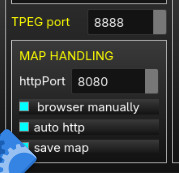
\includegraphics[width=40mm]{tpeg-port.png}
\end{center}

\paragraph{Managing background services}
So, it is easy to start one or more packet services, their running is usually
invisible, since they are running in the background. An exception is the
EPG/SPI service, if that is running, an indicator on the main GUI window
will indicate that.

While not being a packet service, there are cases that audio services are
running as background service as well. Clicking with the {\em right hand} mouse
button on the name of an audio service in the services list tells Qt-DAB to
start that service as background service, writing the MP2 or AAC output into a
file (it does not make much sense to send the output of such a service to
the soundcard).

The - again - {\em configuration and control} window shows the number of
active threads, running services.

\begin{center}
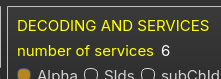
\includegraphics[width=40mm]{servicecount.png}
\end{center}

{\em Clicking} on the number controls the visibility of a small window
showing all running services

\begin{center}
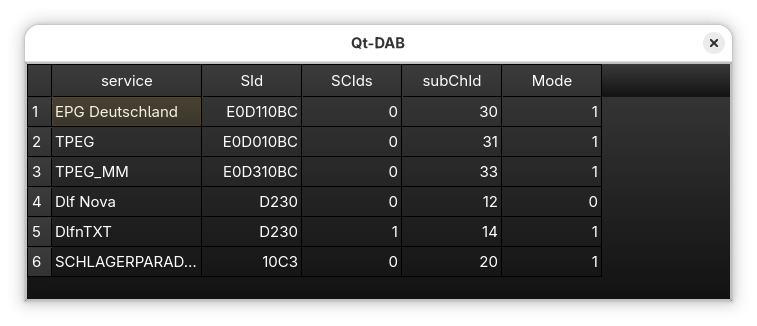
\includegraphics[width=100mm]{background-control.png}
\end{center}

The window shows the services, their SId (the service identification) and
the SCIds (the component number within the service), the subchannel (defining
the format for running), and, finally, the {\em Mode}.
The services for which the SCIds is not 0, are {\em secondary services},
it shows that they share the SId with a primary service.
The Mode is simple, 0 stands for running as foreground service, the 1 stands
for running as background service.

The list shows two primary audio services, {\em Dlf Nova} and 
{\em SchlagerParade}. The first one carries a subservice (a journaline text
service).
The second one has a Mode 1, showing that that
service is running as background service and its audio data is written as
AAC data into a file.

Processing of a service, {\em running in the background}, can be stopped by
clicking with the mouse on the service name in this {\em control} window.
\end{document}
